\chapter{Theoretische Grundlagen}
\label{background}

%- Allgemeine Wissensgrundlagen des Fachgebiets
%- Spezielle Grundlagen, die für das Verständnis erforderlich sind
%- Rahmenbedingungen für die Arbeit
%- Ausführungen zum Stand des Wissens / der Technik
%Als Leitprinzip gilt: Nur Informationen erwähnen, die
%- später benötigt werden,
%- notwendig sind, um die Arbeit oder ihre Motivation zu verstehen
%Das heißt insbesondere,
%- keine Inhalte aus Lehrbüchern, außer
%- diese werden benötigt, um Problemstellung oder Lösungsweg zu definieren.

Ziel des nachfolgenden Kapitels soll es sein, eine allgemeine Wissensgrundlage über wesentliche Begrifflichkeiten im Thema zu schaffen. Um die nachfolgenden Ausführungen im Hauptteil (vgl. \ref{problemfields} und \ref{agilepractices}) besser nachvollziehen zu können, sollen wichtige Definitionen und Begriffsabgrenzungen vorgenommen werden.

\section{Digitale Transformation}
\label{background:dt}

Der wesentliche Schwerpunkt der vorliegenden Arbeit dreht sich um die sogenannte \textit{Digitale Transformation}. Eine allgemeine Definition für diese Begrifflichkeit ist momentan schwer zu finden \cite[S. 3]{schallmo_digitale_2017}. Grundsätzlich versteht man unter der Digitalen Transformation von Unternehmen den Einfluss neuer Technologien und Innovationen auf gesamtunternehmerische Strukturen, Geschäftsmodelle und Wertschöpfungsketten \cite{oswald_digitale_2018}. Nach \citeA{kofler_digitale_2018} sei es das Ziel der digitalen Transformation, Unternehmen fortlaufend und ohne vorhersehbares Ende so umzubauen, dass sie sich den kontinuierlichen Marktveränderungen durch Digitalisierung stellen können (S. 1). Man erkennt hierbei das Muster, dass die Begrifflichkeit der \textit{Digitalisierung} ein wichtiger Faktor für den strategischen Aufbau von Unternehmen geworden ist. Neue Innovationen im digitalen Bereich machen es vor allem kleineren Firmen einfacher in bestehende Märkte einzutreten und sogenannte \textit{Disruptionen} \todo{Erklärung als Fußnote} zu erschaffen. 
 
 
 Viele Versuche einer Definition betreffen immer den Bezug auf aufkommende digitale Technologien. Diese können als sogenannte \textit{Treiber} der Digitalen Transformation bezeichnet werden \cite[S.20]{bloching_digitale_2015}. \ref{fig:bigpicture} skizziert eine Übersicht dieser verschiedenen Treiber. Man erkennt hierbei schon wichtige Handlungsfelder des Transformationsprozess, wie beispielsweise die Automatisierung von Geschäftsprozessen oder die Nutzung von generierten Digitalen Daten. Solche Handlungsfelder werden in der vorliegenden Arbeit in \ref{problemfields:changepatterns} genauer erläutert.
 
\ref{fig:bigpicture} kennzeichnet außerdem, dass eine große Reihe von neuen Technologien die Digitale Transformation antreiben. Beispielsweise bilden Technologien wie \textit{Cloud Computing} oder \textit{Big Data} neue Möglichkeiten für digitalisierte Geschäftsmodelle. 
 
\begin{figure}[H]
	\centering
	\fbox{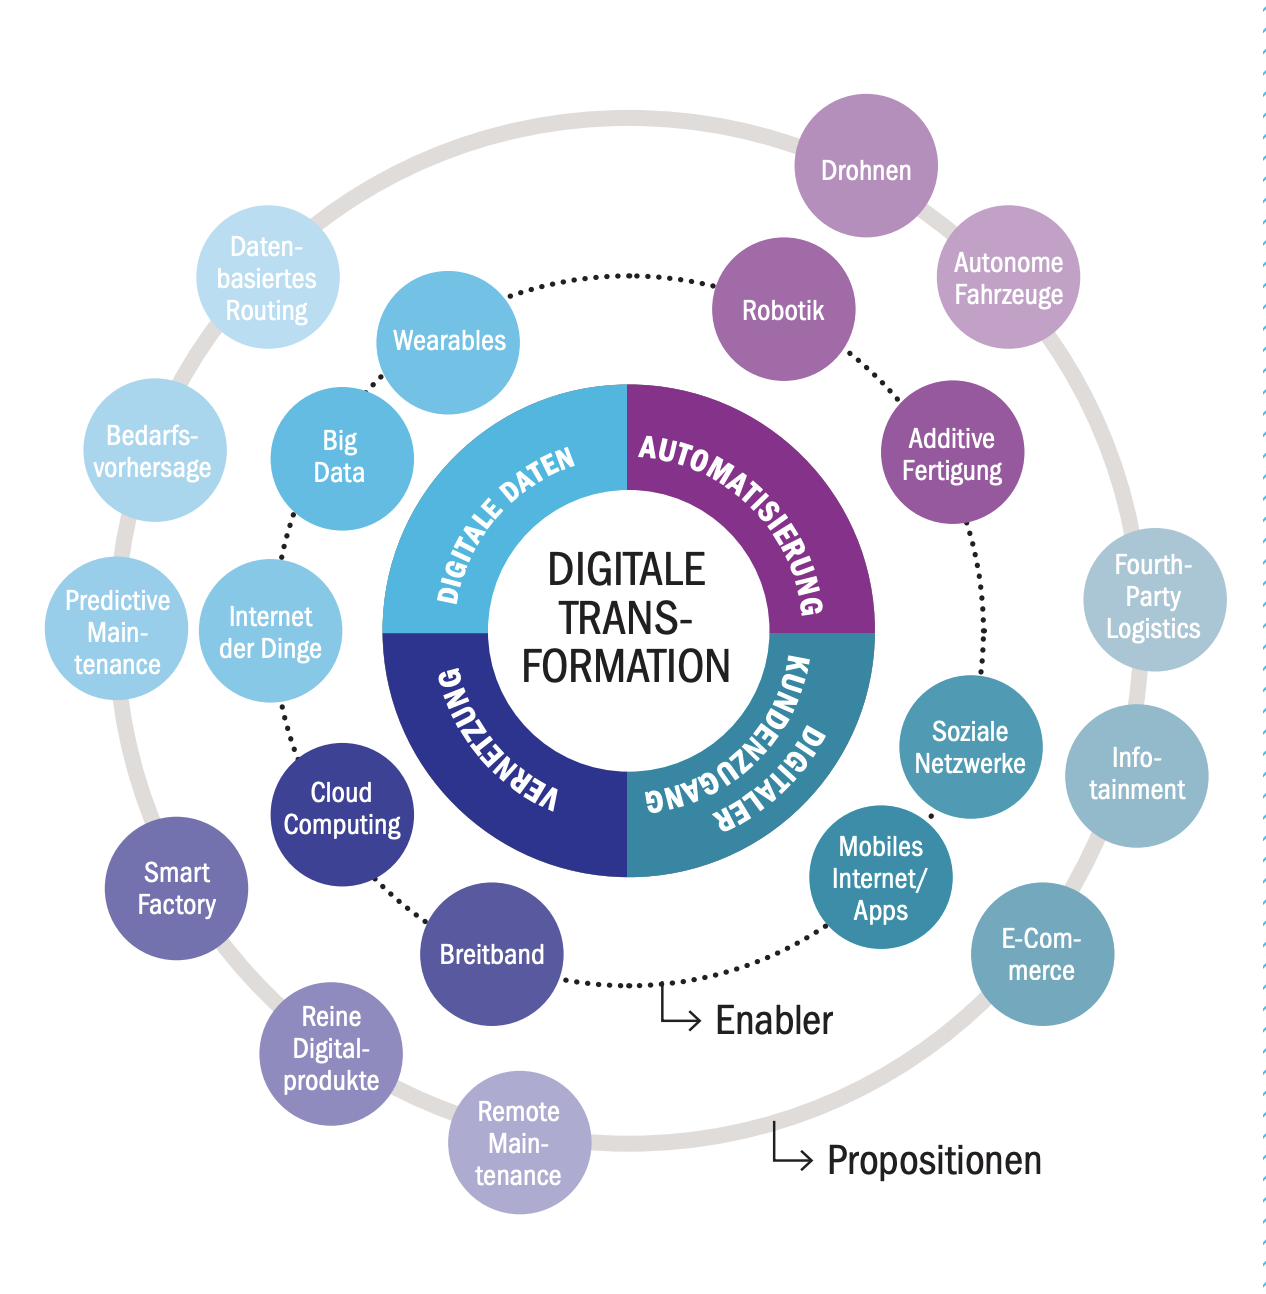
\includegraphics[width=0.7\linewidth]{pics/dtbigpicture}}
	\caption[Big-Picture der Digitalen Transformation]{Treiber der Digitalen Transformation \protect \cite[S. 20]{bloching_digitale_2015}}
	\label{fig:bigpicture}
\end{figure}

Die Digitale Transformation kann somit als weitreichender Veränderungsprozess von Unternehmen angesehen werden. \citeA{oswald_digitale_2018} beschreiben innerhalb dieses Prozesses vier bestimmende Charakteristika. Demnach sei die Digitale Transformation ''unausweislich, unumkehrbar, ungeheuer schnell und mit Unsicherheit behaftet`` (S. 10). Man erkennt hierbei also ein gewisses Risiko bei der Bearbeitung einer solchen Transformation. Es ginge für das Unternehmen vor allem darum, ''die Chancen neuer, digitaler Technologien kontinuierlich hinsichtlich ihres Potentials zur Weiterentwicklung bestehender Geschäftsmodelle zu evaluieren`` (S. 10).

Es kristallisiert sich ganz klar heraus, dass der Veränderungsprozess einer Digitalen Transformation zwar unausweichlich ist, um die eigene Marktposition zu verteidigen. Trotzdem zeigen sich zunehmende Risiken und Probleme bei der Implementierung solcher Veränderungen. Demnach liegt es nahe, sich in der vorliegenden Arbeit mit den Problemfeldern der Digitalen Transformation zu beschäftigen (vgl. \ref{problemfields}).

\section{Change Management}

\begin{figure}[h]
	\centering
	\fbox{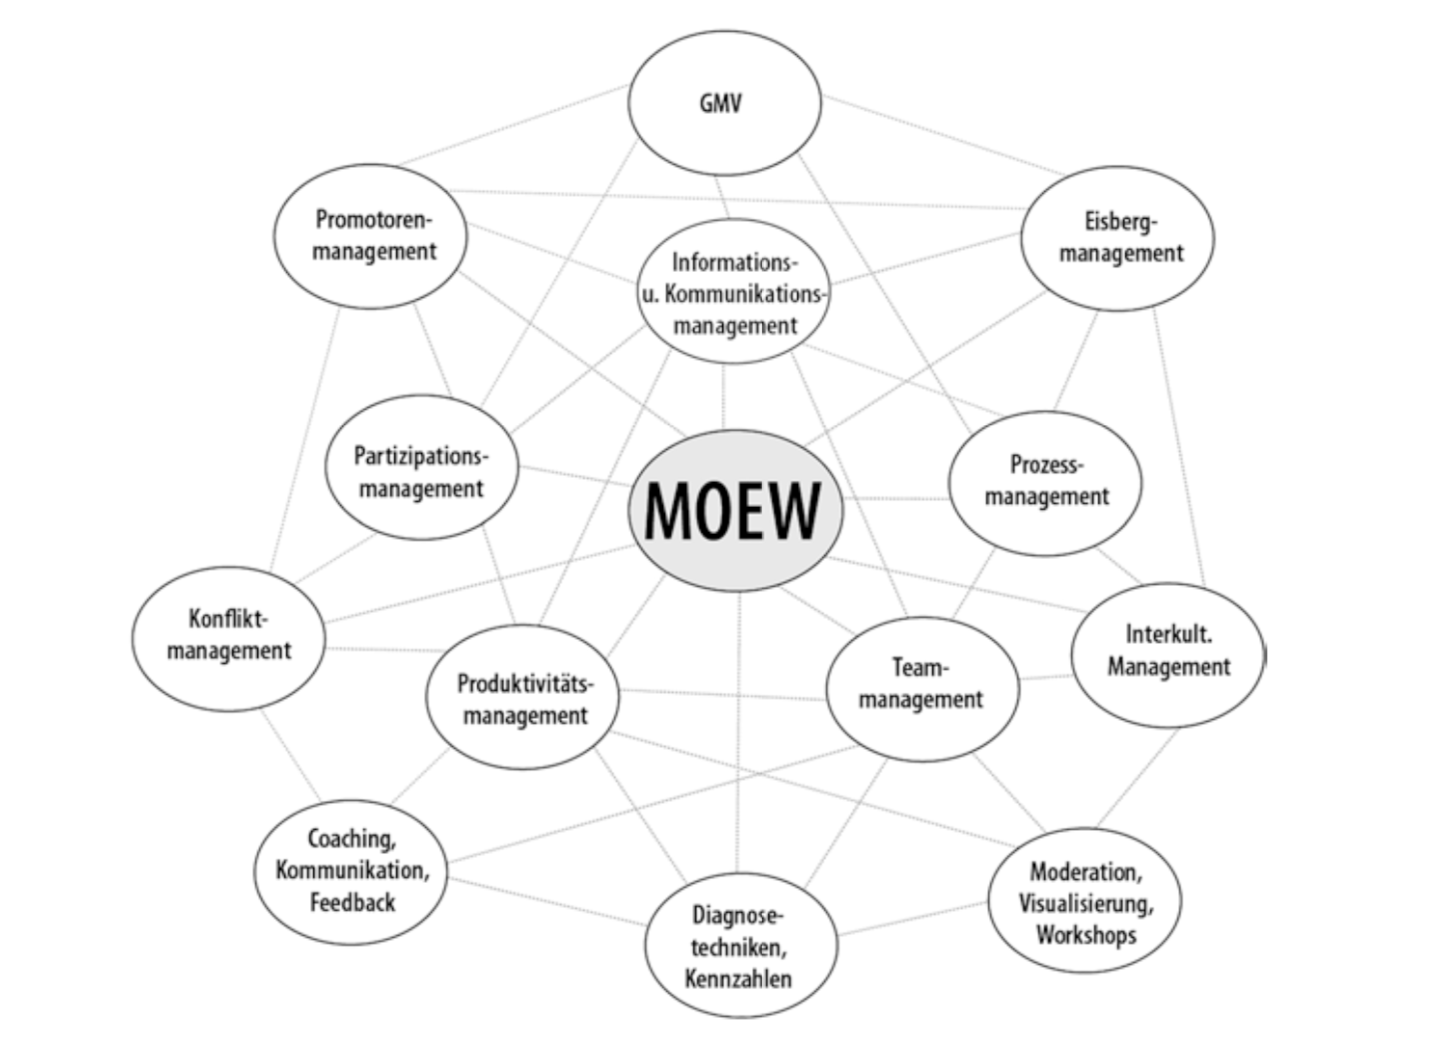
\includegraphics[width=0.7\linewidth]{pics/moew}}
	\caption[Bestandteile des MOEW-Modells]{Bestandteile des MOEW-Modells \protect \cite[S. 12]{kaune_change_2016}}
	\label{fig:moew}
\end{figure}
\todo{eventuell Bild verbessern}

Wie im vorhergehenden Abschnitt bereits angeklungen ist, handelt es sich bei der Digitalen Transformation um einen großangelegten Veränderungsprozess eines Unternehmens. Vordergründig kann definiert werden, dass es sich beim Veränderungsmanagement bzw. \textit{Change Management} um das ''$\lbrack$m$\rbrack$anagen von Veränderungen in Unternehmen und Organisationen`` \cite[S. 10]{kaune_change_2016} handelt. Durch die gravierenden Änderungen des Unternehmens und die Notwendigkeit, einen geordneten Veränderungsprozess anzustoßen, kann das Steuern der Digitale Transformation grundsätzlich als Change Management bezeichnet werden. Die Transformation muss gezielt gesteuert werden, eine eigenes Management-Konzept ist unabdingbar um den Herausforderungen entgegenzuwirken \cite[S. 19]{hess_digitale_2019}. Nachfolgend sollen in kurzer Form verschiedene Change-Management-Ansätze gezeigt werden, um ein generelles Verständnis über diese Problematik zu erhalten.

Eine generelle Definition für die Begrifflichkeit konnte in den vorangestellten Ausführungen bereits aufgestellt werden \cite{kaune_change_2016}. Grundsätzlich können Veränderungsprozesse \textit{top-down} (z.B. Business Reengineering), d.h. revolutionär, von der oberen Managementabteilung zentral voran geführt; oder \textit{bottom-up} (z.B. Organisationsentwicklung), d.h. evolutionär, die Mitarbeiter stark einbindend; geprägt sein \cite[S. 10]{kaune_change_2016}. Soll eine Veränderung ''sozial und ökonomisch nachhaltig wirksam sein``, so \citeA{kaune_change_2016}, sei eher der zweite Ansatz zu wählen, da ''über
das Einbeziehen und die aktive Einbindung der Mitarbeiter Identifikation mit dem Veränderungsobjekt geschaffen wird`` (S. 11). Wie in \ref{background:dt} bereits angeklungen, dass eine kontinuierliche Lösung innerhalb der Digitalen Transformation Vorteile haben kann. Allerdings spricht man bei den vorzunehmenden Veränderungen von ''ungeheuer schnell``  \cite[S. 10]{oswald_digitale_2018} , so dass ebenfalls revolutionäre Ansätze einzusetzen wären. Ob und inwieweit die genannten Ansätze Einklang in einen Change-Management-Prozess für die Digitale Transformation von Großunternehmen finden, soll im weiteren Verlauf dieser Arbeit geklärt werden.

Als ein wesentlicher Punkt des Change Management innerhalb einer Digitalen Transformation wird die Einbeziehung der Mitarbeiter des Unternehmens genannt \cite[S. 179f.]{hess_digitale_2019}. \citeA{kaune_change_2016} beschreiben in ihren Ausführungen das sogenannte \textit{MOEW-Modell} (Moderne Organisationsentwicklung) als ein Ansatz der partizipativen Organisationsentwicklung (S. 11). Ohne zu genau auf die einzelnen Bestandteile einzugehen, zielt das Modell auf eine ''gleichzeitigen Verbesserung der Leistungsfähigkeit der Organisation und der Qualität des Arbeitslebens`` (S. 11) ab. Dabei werden verschiedenste Komponenten des Veränderungsmanagement, beispielsweise Partizipations-, Prozess- oder Kommunikationsmanagement, sowie eine Reihe von Tools und Techniken eng miteinander verknüpft werden, um Mitarbeiter direkt in den Veränderungsprozess mit einzubinden und einen langfristigen Erfolg zu erzielen (S. 11f.). \ref{fig:moew} zeigt die einzelnen Bestandteile des MOEW-Modells.

Die Einbindung und Beurteilung der Mitarbeiter des Unternehmens hat eine große Bedeutung im Veränderungsprozess inne. Den Menschen in den Mittelpunkt zu stellen ist ein wichtiges Erfolgskriterium, da jede Veränderung zwangsläufig immer den Menschen direkt betrifft \cite[S. 3]{bertagnolli_change_2018}. \ref{fig:changekurve} illustriert die sogenannte \textit{Change-Kurve} und gibt einen Überblick darüber, inwieweit sich das Verhalten von Mitarbeitern in einem Change-Management-Prozess verändert. ''Werden Menschen in Veränderungen nicht aktiv eingebunden oder nicht beachtet, wird der auftretende Widerstand noch stärker und letztendlich zu einer Blockade``, so \citeA{bertagnolli_change_2018} (S. 3f.). Ziel eines jeden Veränderungsprozesses solle es sein, Widerstand zu bearbeiten und möglichst zu beseitigen (ebenda). 

 \begin{figure}
	\centering
	\fbox{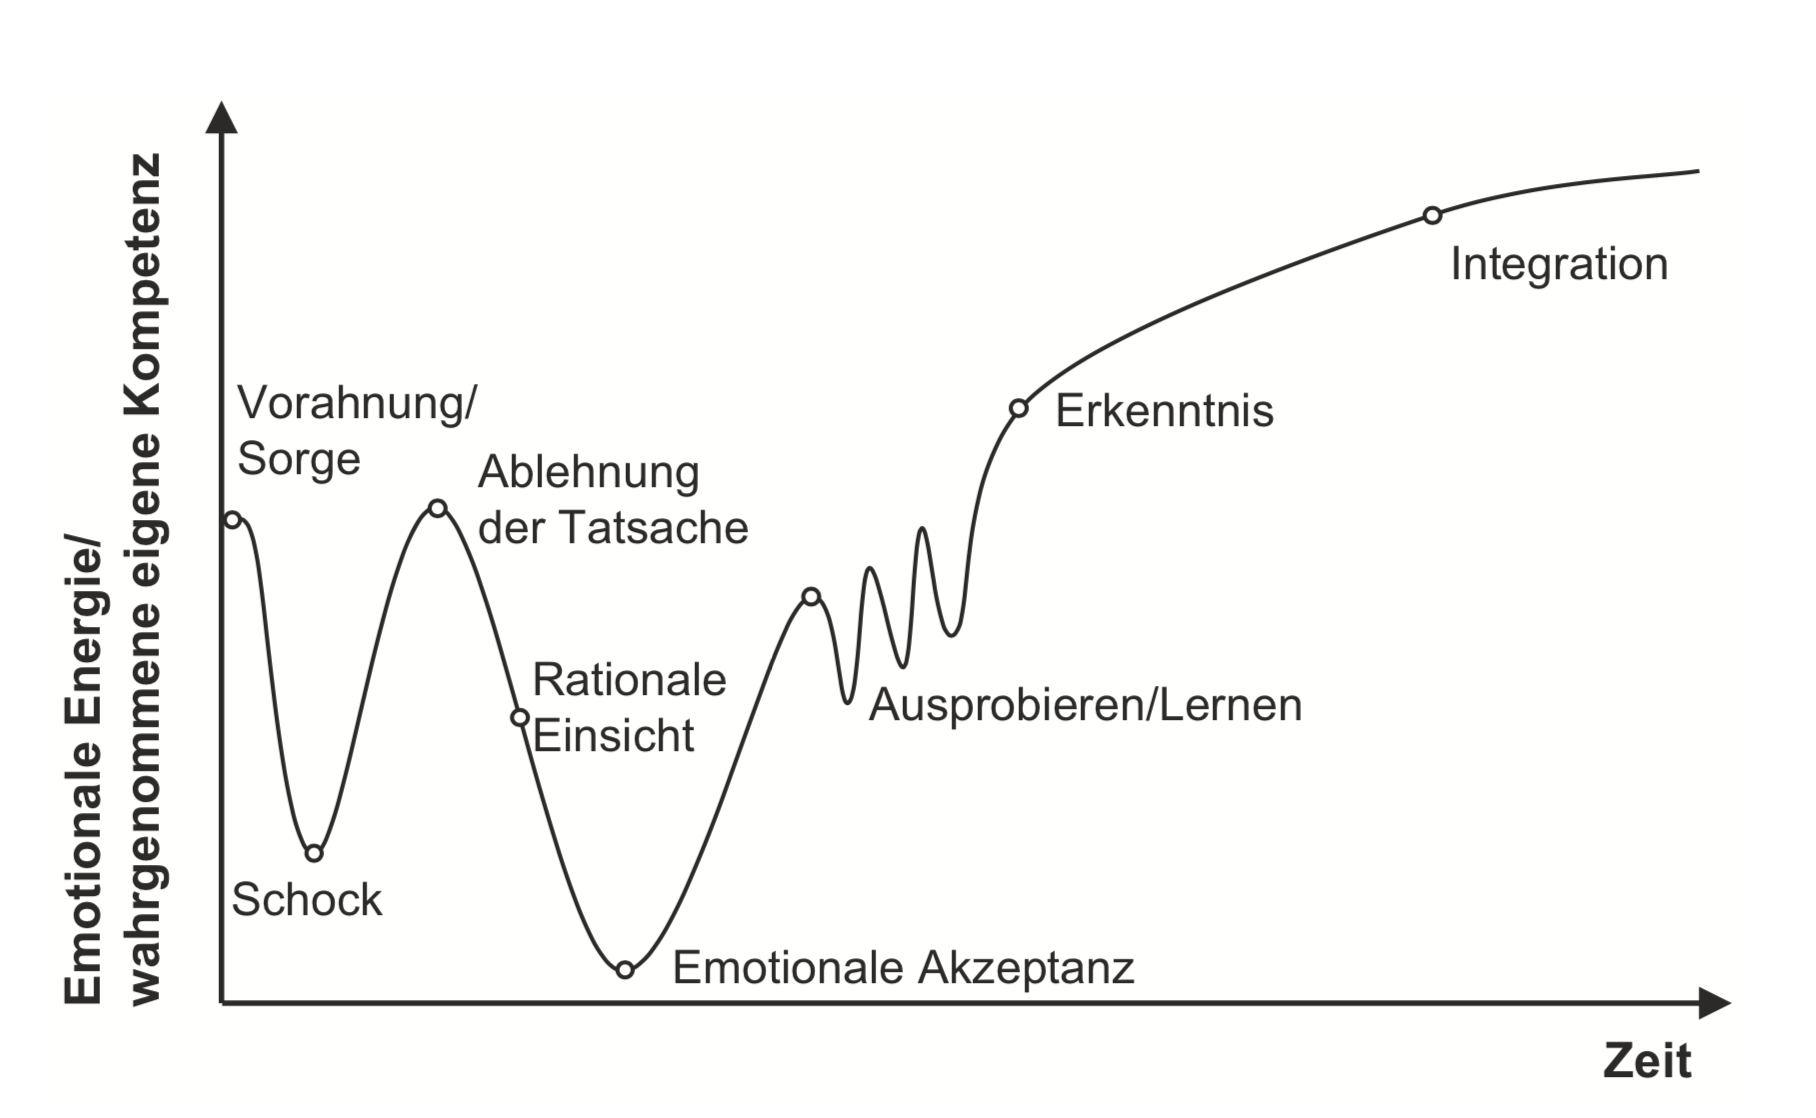
\includegraphics[width=0.8\linewidth]{pics/changekurve}}
	\caption[Change-Kurve von Mitarbeiterverhalten]{''Change-Kurve``: Veränderungsverhalten von Mitarbeitern \protect \cite[S. 3]{bertagnolli_change_2018}}
	\label{fig:changekurve}
\end{figure}

Neben den einzelnen Komponenten des Change Managements finden außerdem ausgewählte Werkzeuge Eingang in den Veränderungsprozess. Das genannte MOEW-Modell führt erste Beispiele auf, wie beispielsweise Coaching und Workshops. Neben diesen finden aber auch andere Techniken weite Anwendung. Ohne dem nächsten \ref{background:agile} etwas vorwegzunehmen, können hier Agile Methoden genannt werden, welche ebenfalls einen wesentlichen Schwerpunkt der vorliegenden Arbeit bilden. Gerade im Hinblick auf die Einbindung von Mitarbeitern erfreuen sich solche Praktiken großer Beliebtheit. Nach \citeA{olbert_uberlebenselixier_2019} sei es wichtig, ''Betroffene zu Beteiligten [zu] machen``, um damit zu erreichen, ''dass die vom Wandel Betroffenen nicht Objekte von Top-down-Entscheidungen, sondern Mitgestalter des
Wandels sind`` (S. 6). 

Die Verbindung der Agilität mit Change Management macht aus diesen Gesichtspunkten also durchaus Sinn. Deswegen erscheint für die vorliegende Arbeit die Einwirkung von Agilen Methoden in den Transformationsprozess als ein interessantes Untersuchungsgegenstand. Aus diesem Grund soll im folgenden ein kleiner Umriss über das Thema der Agilität gegeben werden.

\section{Agilität}
\label{background:agile}

Der Begriff  \textit{Agilität} in dem Kontext wie er in der vorliegenden Arbeit thematisiert wird liegt der Agilen Softwareentwicklung zu Grunde. Begründet wurde diese grundlegend im Jahre 2001 von einer Reihe erfahrener Softwareentwickler im sogenannten \textit{Agilen Manifesto} \cite{beck_manifesto}. Diese legten in eben diesem zudem vier wichtige Leitlinien der Agilen Softwareentwicklung fest (übersetzt aus dem Original):

\begin{itemize}[noitemsep, topsep=0pt]
	\item Individuen und Interaktionen stehen über Prozessen und Werkzeugen
	\item Funktionierende Software steht über einer umfassenden Dokumentation
	\item Zusammenarbeit mit dem Kunden steht über der Vertragsverhandlung
	\item Reagieren auf Veränderung steht über dem Befolgen eines Plans
\end{itemize}

Man erkennt hierbei sehr gut, dass ein wesentlicher Bestandteil Flexibilität und Reaktionsfähigkeit auf Veränderungen sind. Wichtige Fähigkeiten im Bezug der Digitalen Transformation \todo{Zitat?} Diese Prinzipien der Agilen Softwareentwicklung lassen sich ebenfalls auf größere Organisationen ausweiten. Nach \citeA{hofert_agiler_2016} ist ''Agilität [...] die Fähigkeit von Teams und Organisationen, in einem unsicheren, sich veränderndem und dynamischen Umfeld flexibel, anpassungsfähig und schnell zu agieren.`` (S. 5). Auf den genauen Begriff der \textit{Agilen Organisation} wird im  folgenden \ref{background:agileorganisation} noch eingegangen. Zunächst sollen weitere Schwerpunkte der Agilität definiert werden.

Neben den bereits aufgeführten agilen Leitlinien sind außerdem sogenannte \textit{Agile Werte}, \textit{Prinzipien} und \textit{Methoden}. Letzteres soll im folgenden nicht weiter ausgeführt werden, da Agile Methoden noch in \ref{agilepractices} detailliert aufgeführt werden. Zu erwähnen sei zunächst nur, dass solche als ``gebündelte Handlungen und in Konzepte übersetzte Aktionen, die auf den agilen Prinzipien beruhend oder in einem anderen Kontext entwickelt wurden, aber zum agilen Denken passen'' \cite[S. 17]{hofert_agiler_2016}.

Agile Werte gehören deshalb zu einem jeden erfolgreichen, agilen Prozess, weil sie die Haltung eines jeden Beteiligten direkt beeinflussen. Sie sorgen indirekt dafür, dass sich Mitarbeiter für ein Vorhaben besonders motivieren können \cite[S. 10]{hofert_agiler_2016}. Gerade in einem groß ausgelegten Veränderungsprozess wie die Digitale Transformation können solche Werte zu einer besseren Bekämpfung von Widerstand beitragen. Verschiedenste Literatur definieren  unterschiedliche Grundtypen agiler Werte und sicherlich muss jedes agile Vorhaben diese neu erläutern. Grundsätzlich können folgende agile Werte aufgeführt werden  (nach \citeA{hofert_agiler_2016}, S. 11):

\begin{itemize}[noitemsep, topsep=0pt]
	\item Selbstverpflichtung (Commitment)
	\item Rückmeldung (Feedback)
	\item Fokus (Focus)
	\item Kommunikation (Communication) 
	\item Mut (Courage)
	\item Respekt (Respect)
	\item Einfachheit (Simplicity)
	\item Offenheit (Openness)
\end{itemize}

Aus eben diesen können sogenannte Agile Prinzipien abgeleitet werden. Diese kann man als eine Art \textit{Spielregeln} im Teamkontext verstehen. Während sich agile Werte also auf jeden einzelnen beziehen, können Prinzipien eher als zwischenmenschliche Aspekte verstanden werden \cite[S. 12]{hofert_agiler_2016}. Nach \citeA{hofert_agiler_2016} soll die folgende \ref{tab:agileprinzipien} soll eine Reihe von Beispielen für agile Prinzipien und die darauf zugrunde liegenden Werte geben.

\begin{table}[htbp]
	\caption{Beispiele agiler Prinzipien}
	\begin{center}
			\begin{tabular}{|c|c|}
				\hline
				\textbf{Prinzip} & \textbf{zu Grunde liegender agiler Wert}\\
				\hline
				Adaption & Einfachheit \\
				Aktive Einbindung & Kommunikation\\
				Bevollmächtigtes Team & Selbstverpflichtung \\
				Experimentieren & Mut, Rückmeldung \\
				Iteration &  Einfachheit \\
				Kontinuierliche Verbesserung & Einfachheit, Fokus, Selbstverpflichtung \\
				Sagen statt Fragen & Offenheit, Kommunikation \\
				Vielfalt & Respekt \\
				Zusammenarbeit aller Beteiligten & Kommunikation, Rückmeldung \\
				\hline
			\end{tabular}
		\label{tab:agileprinzipien}
	\end{center}
\end{table}

\todo{Big picture agile selbst erstellen?}

Natürlich gibt es zunehmend Abwandlungen für die Anwendung von Agilität in bestimmten Prozessen. Dafür ist die Begrifflichkeit nicht eindeutig definiert. Die agilen Prinzipien können aber einen Anhaltspunkt dafür geben, wie Change Management Prozesse positiv  beeinflusst werden können. Wie und inwieweit bestimmte agile Methoden dazu beitragen können, wird in \ref{agilepractices} noch ausführlich erläutert.

\todots

\section{Agile Organisation}
\label{background:agileorganisation}

\todo{Kurz, mit Bezug auf vorangegangen Abschnitt}

\todots

\section{Agile Transformation}

\todots

\section{Abgrenzung Großunternehmen}

Wie den Forschungsfragen zu entnehmen konzentriert sich die zu erstellende Arbeit auf \textit{Großunternehmen}. Dies liegt unter anderem dem aktuellen Forschungsstand zu Grunde. Bisher weitreichende Studien zur Digitalen Transformation beschäftigen sich vermehrt mit größeren Unternehmen. Dies hat zur Folge, dass die Untersuchung der zu erstellenden Arbeit auf eine größere Literaturbasis zurückgreifen kann. Eine entsprechende Abgrenzung zu kleinen und mittelständischen Unternehmen (KMU) soll nun vorangestellt werden.

Als Grundlage für die spätere Literatursuche in den Kapiteln 4 und 5 muss die Begrifflichkeit  des Großunternehmens  klar definiert werden, um sie von anderen Unternehmensarten wie KMU abzugrenzen. Es gibt eine Reihe von möglichen Definitionen aus verschiedenen Quellen. In der vorliegenden Arbeit soll die Definition der EU-Empfehlung 2003/361/EG \footnote{Empfehlung der Kommission vom 6. Mai 2003, betreffend die Definition der Kleinstunternehmen sowie der kleinen und mittleren Unternehmen, online: $\url{https://eur-lex.europa.eu/legal-content/DE/TXT/PDF/?uri=uriserv:OJ.L_.2003.124.01.0036.01.DEU}$} genutzt werden. Demnach gelten solche Unternehmen als Großunternehmen, welche mehr als 250 Mitarbeitern oder einem Jahresumsatz über 50 Millionen Euro verbunden mit einer Bilanzsumme über 43 Millionen Euro aufweisen.

Selbstverständlich können andere Definitionen gewählt werden, wie beispielsweise aus dem deutschen Handelsrecht \footnote{ § 267 HGB, § 221 UGB}. Die Vorgabe nach europäischem Recht kann aber als gute Grundlage für die nachfolgende Benutzung der Begrifflichkeit des Großunternehmens genutzt werden. Eine international gültige Definition gibt es nicht. An dieser Stelle sei vermerkt, dass die nachfolgende Literatursuche in den Kapiteln 4 und 5 nicht nur europäische Großunternehmen einschließt. Die Methodikteile der jeweiligen Kapitel werden darauf noch gesondert eingehen.